\documentclass[journal,12pt,twocolumn]{article}
\usepackage[english]{babel}
\usepackage[letterpaper,top=2cm,bottom=2cm,left=3cm,right=3cm,marginparwidth=1.75cm]{geometry}
\usepackage{multicol}
%\usepackage{amsmath}
\usepackage{graphicx}
%\usepackage{array}
\usepackage{blindtext}
\usepackage[utf8]{inputenc}
\usepackage{watermark}
\usepackage{hyperref}
\usepackage{fancybox}
%\usepackage[colorlinks=true, allcolors=blue]{hyperref}
\usepackage{listings}
\usepackage{float}

\title{FM}
\author{Under guidance of Dr.GVV SHARMA}
\thiswatermark{\centering \put(-50,-105){
\includegraphics[scale=0.5]{iith.png}}}

\begin{document}
\maketitle
\tableofcontents

\section{Project Abstract}
Finding the bandwidth of an audio signal which is .wav file.

\section{Audio Signal}
	When working with audio files, it is important to consider the following information:

\begin{enumerate}
\item{\textbf{Format:}

	The format of the audio file specifies how the audio data is encoded and stored. Common audio formats include WAV, MP3, FLAC, and AAC.}
 
\item{\textbf{Sample Rate:}

	The sample rate of an audio file specifies how many samples of the audio signal are taken per second. It is typically measured in Hertz (Hz), and common sample rates include 44.1 kHz, 48 kHz, and 96 kHz.}
 
\item{\textbf{Depth} 

	The bit depth of an audio file specifies the number of bits used to represent each sample of the audio signal. Higher bit depths allow for greater precision in representing the audio signal, but also result in larger file sizes. Common bit depths include 16-bit and 24-bit.}

\end{enumerate}

	Understanding these properties of an audio file is important for analyzing and processing the audio data. 


\section{Loading the Audio file}
	We begin by loading the audio file using the wavfile.read() function from the scipy.io.wavfile module. This returns the sampling frequency and the audio data as a numpy array.


\section{Computing the Fourier Transform}
	The Fourier transform of the audio signal using the numpy.fft.fft() function. This transforms the audio data from the time domain to the frequency domain.

\begin{figure}[h]
    \centering
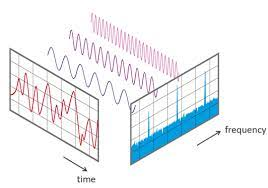
\includegraphics[width=\columnwidth]{fft.jpeg}
    \label{fig:my_label}
\end{figure}

\vspace{2cm}
 
	The FFT algorithm is widely used in signal processing, digital image processing, audio processing, and other fields where data is represented in the form of a sequence of samples. By using the FFT algorithm, it is possible to analyze and manipulate the frequency content of a signal, which can be useful for tasks such as filtering, compression, and feature extraction. 	
\begin{figure}[h]
    \centering
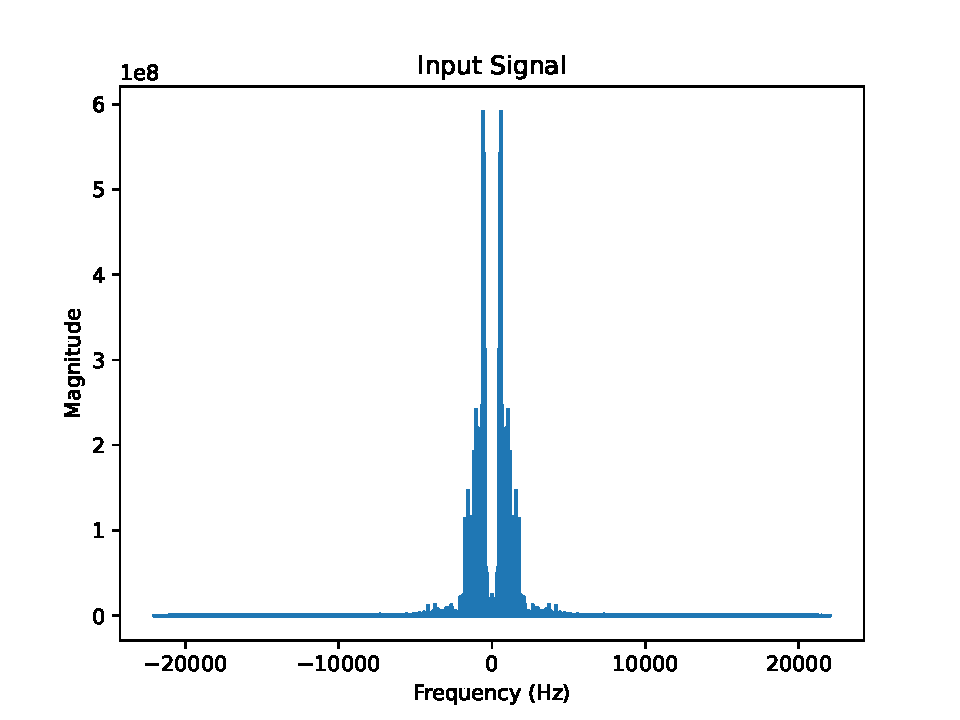
\includegraphics[width=\columnwidth]{input.pdf}
    \label{fig:my_label}
    \caption{Spectrum of audio signal}
\end{figure}


\section{Bandwidth}
	Bandwidth refers to the range of frequencies or the frequency band over which a signal or a system can effectively transmit or process information with acceptable quality, without significant distortion or loss of information.

	Bandwidth is of primary importance in communication system as the available bandwidth is limited , engineers are developing sytems which uses least possible bandwidth.

Bandwidth can de defined as:
\begin{enumerate}

\item{\textbf{Spectral Analysis:}

	The bandwidth of a signal can be determined from its frequency spectrum, which shows the amplitude of the signal at different frequencies. The bandwidth can be calculated as the difference between the highest and lowest frequencies that contain significant signal energy, typically defined as the frequency range where the signal amplitude is above a certain threshold. The frequency spectrum can be obtained using tools such as the Fourier transform or the power spectral density function.}

\item{\textbf{Half power or -3db method:}

	The difference between the limiting frequencies is called the bandwidth, and is expressed in hertz.The limiting frequencies of a passband are defined as those at which the relative intensity or power decreases to a specified fraction of the maximum intensity or power. This decrease in power is often specified to be the half-power points, i.e., 3 dB below the maximum power.}

\item{\textbf{Carson's rule:}

	Carson's rule is a simplified approximation for calculating the bandwidth of an FM signal. According to Carson's rule, the bandwidth of an FM signal is approximately equal to twice the sum of the highest frequency deviation (${\Delta}$f) and the frequency of the modulating signal (fm). Mathematically, bandwidth = 2(${\Delta}$f + fm).}

\item{\textbf{Nyquist-Shannon sampling theorem:}

	The Nyquist-Shannon sampling theorem states that the sampling rate of a digital signal must be at least twice the highest frequency component in the signal in order to avoid aliasing. The bandwidth of the signal can be calculated as half of the sampling rate.}

\end{enumerate}


\section{Bandwidth Calculation}
	We are calculating bandwidth by first method i.e., by spectral analysis using power spectral density function.
	
	The power spectral density (PSD) is a measure of the power of a signal as a function of frequency. 
	
\begin{enumerate}

\item{We first load the WAV file using SciPy's \textbf{wavfile.read()} function, which returns the sample rate and signal as separate variables.}
	
\item{We then perform an FFT on the signal using NumPy's \textbf{fft} function. Next, we calculate the power spectral density (PSD) of the signal by taking the absolute value of the FFT and squaring it.} 
	
\item{We also calculate the frequency range using NumPy's \textbf{fftfreq} function, with the sampling interval set to \textbf{1/sample\_rate} to account for the sample rate of the audio file.} 
	
\item{Finally, we find the frequency range with significant power by applying a mask to the PSD and computing the minimum and maximum frequencies. The bandwidth is simply the difference between these frequencies.we obtain the bandwidth of the audio as 2 khz}

	
\end{enumerate}
   \section{Code Link}
	The below python code computes bandwidth of the input audio file:
	\vspace{2cm}
    \fbox{\parbox{3cm}{\href{https://github.com/imran111888/fwc2/blob/main/FM/code/input.py}{input.py}}}

\end{document}
